\section{Introduction[Skip please]}
Thanks to the potential application prospects of Human Activity Recognition(HAR)in security, virtual reality, sports training and health care[2], it has become a very hot and interesting research field for the machine-learning community in the past decades. It takes advantage of data coming from internal sensors like accelerator and gyroscope to automatically classify user activities. Since the structure of data coming from sensors is stochastic over time, in order to classify them, we have to apply one of the time series classification techniques such as sliding window.

\section{Background}
\subsection{Activity recognition process}\label{subsec:ARP}

% figure 2
\begin{figure}[h]
    \centering
    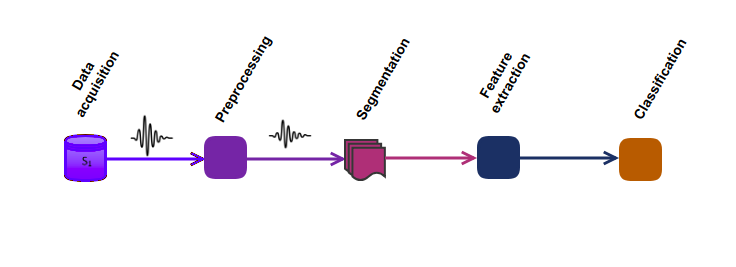
\includegraphics[width=.5\textwidth]{Figures/HARP.png}
    \caption{Time Series classification process through sliding window approach}
    \label{fig:tsprocess}
\end{figure}




An Activity Recognition Process (ARP), also known as the activity recognition chain, is a sequence of signal processing, pattern recognition, and machine learning techniques that implements a specific activity recognition system behavior \cite{bulling2014tutorial}. This method consists of 5 steps which are shown in Figure \ref{fig:tsprocess} and is explained precisely in this section.
\begin{itemize}
\item \textbf{Data acquisition:}There are several sensors attached to various parts of one's body which transform his or her performing action to a set of signals and transmit them to the receiver(s). 
\item \textbf{Preprocesing:} The submitted data from sensors may be disrupted by artifacts caused
by a variety of sources such as electronic fluctuations, sensor malfunctions, and physical activities. In order to eliminate such artifacts, we can apply varying kind of filtering process like the low-pass filter which was applied in some studies \cite{morris2014recofit}. It should be noted that applying these filters may result in removing some valuable information from the signals. 

% figure 2

\begin{figure}[h]
    \centering
    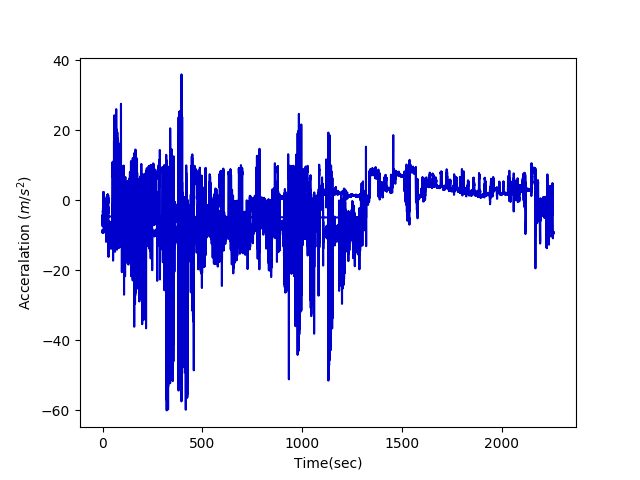
\includegraphics[width=.4\textwidth]{Figures/signal.png}
    \caption{Example of data coming from the x dimension of accelerator in the dataset for subject 1  }
    \label{fig:signal}
\end{figure}

\item \textbf{Segmentation:}
As Figure \ref{fig:signal} indicates, there is a kind of motion in the signals and to capture it, the signals are partitioned into several parts (windows). The label (activity)of each window is the most frequent activity. The number of data points (window size) in each window is not prior and heavily impacts the performance of classifiers \cite{bulling2014tutorial} and different sizes should test to find the optimal window size which is challenging and time-consuming. If each window shares some part of itself with the previous one, it is called overlapping sliding windowing (see Figure \ref{subfig:OSW}).  

\item \textbf{Feature extraction:}
Then each window is transformed into a vector of features ranging from auto-correlation features \cite{morris2014recofit} to time/frequency domain and statistical features which are discriminative for the activities.
\item \textbf{Classification:}
Finally, the Machine Learning classifier is fed by the vector of features and corresponding ground truth activity label to train and assigns the future observations to one of the learned activities or labels.


\end{itemize}



\subsection{Related work} \label{sub:theirwork}
As discussed in the Section \ref{subsec:ARP} opting the number of data-points (window size)in the segmentation stage of the ARP can influence the performance of the classifiers and mostly is selected by trial and error or based on the previous studies. Banos et al \cite{banos2014window} does an extensive study to show such impact and provide a guideline to select the window size.They apply ARP (\ref{subsec:ARP}) on the acceleration data of a very big dataset \cite{banos2012benchmark} which is precisely explained in the Section \ref{sec:dataset}.\cite{banos2014window}segments the signals without any preprocessing by non-overlapping sliding window approach with diverse sizes ranging from .25 s to 7 s in the steps of .25 s.Regarding the feature extraction step, they consider three different feature sets(FS) namely FS1 = {mean}, FS2 ={mean and standard deviation} and FS3 = {mean, standard deviation, maximum, minimum and mean crossing rate}.Most of these features have been used in previous works due to their speed in the calculation and being informative and discriminative over each window. They also take advantage of four machine learning models: C4.5 decision trees (DT), k-nearest neighbors (KNN) with k=3, naive Bayes (NB) and nearest centroid classifier (NCC) to classify the activities and report the F1-score through a ten-fold cross-validation (10-fold XV) process to choose the optimal window size. We build on their work to remove several limitations which are explained in the next section.

\subsection{Motivation for our study}
In this section two significant determinants which are overlooked in \cite{banos2014window} are examined categorically.

\begin{figure}[htp]
  \centering
  \subfigure[Non-overlapping]{
\label{subfig:NOSW}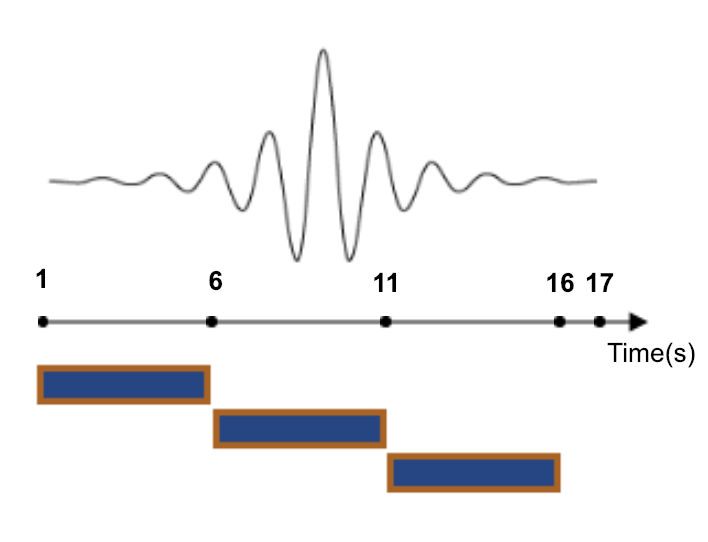
\includegraphics[scale=0.32]{Figures/NOSW.png}}\quad
  \subfigure[Overlapping-2.5 s sharing s]{\label{subfig:OSW}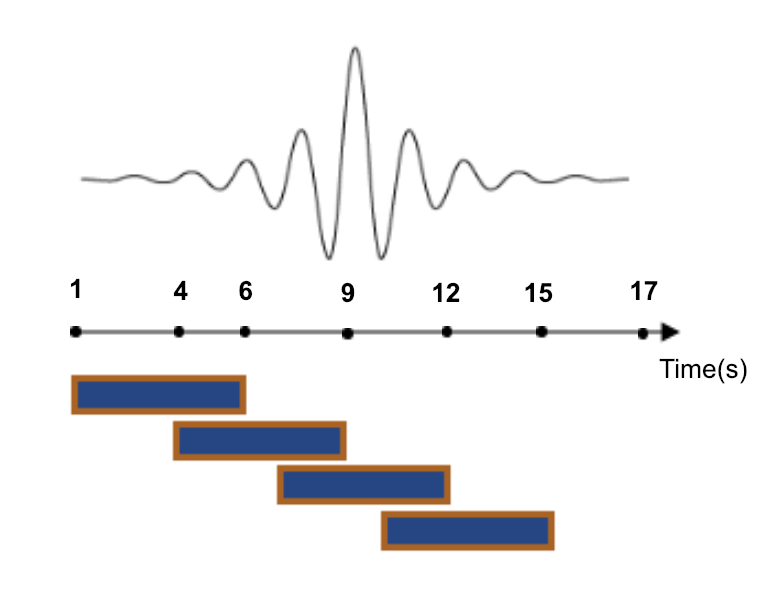
\includegraphics[scale=0.32]{Figures/OSW.png}}

   \caption{5 second sliding window}
   \label{fig:SlidingWindow}
\end{figure}

\begin{itemize}
\item \textbf{Non-overlapping sliding window}:As described in Section \ref{sub:theirwork}, \cite{banos2014window} uses a non-overlapping sliding window technique in the segmentation step of the human activity process.Figure \ref{fig:SlidingWindow} apparently shows the non-overlapping sliding window and overlapping sliding window processes. In segmentation step of ARP, we try to segment the signals so that the data points of each activity settle entirely in a window and also each window contains the observations of only one activity in order to make the features calculation over each window more discriminative.
As can be seen in the \ref{fig:SlidingWindow}, the probability of alighting each activity in a window and having a purer window in \ref{fig:NOSW} is lower than that in \ref{fig:OSW}.To illustrate, consider an activity which starts from t=5s and lasts 10 s.In the non-overlapping approach, the half of data-points settle in the first window and the rest will be in the next window. However, in the overlapping sliding window, the entire activity will be in the second window. On the other hand, the overlapping approach captures more patterns in the signals and leads to more data which usually appropriate for machine learning models. Thus, making decision for any part of the human ARP base on the non-overlapping sliding window may be not accurate.\newline


\item \textbf{Classic K-fold cross-validation (CV) process}:
\cite{banos2014window} applies a 10-fold CV process in order to evaluate the performance of their models.
The main hypothesis of the classic K-fold cross-validation process is that samples are Independent and Identically Distributed (i.i.d.).It means that all the data points sampled from the same distribution and also the distribution has no memory of past generated samples. Under such an assumption, as shown in Figure \ref{fig:Shuffle-cv} the test set can be any part of the dataset. However, we know that samples coming from sensors are characterized to have correlation and the i.i.d. assumption of the CV is violated. Thus, evaluation models through classic CV would result in an illogical choosing of test and training set since the test set can be before the training set which is unreasonable. Although one may claim that after partitioning the dataset into some windows based on the Markov chain \cite{gilks1995markov} they are i.i.d..However, through splitting the dataset by a window size, there is no guarantee to find the best number of samples to make a window completely independent of others. Hence, in order to find the best window size for the segmentation part of ARP based on the performance of classifiers, we should use more realistic cross-validation process such as subject cross-validation process which is explained deeply in Section \ref{sub:subjective CV}.

% figure 3
\begin{figure}[h]
    \centering
    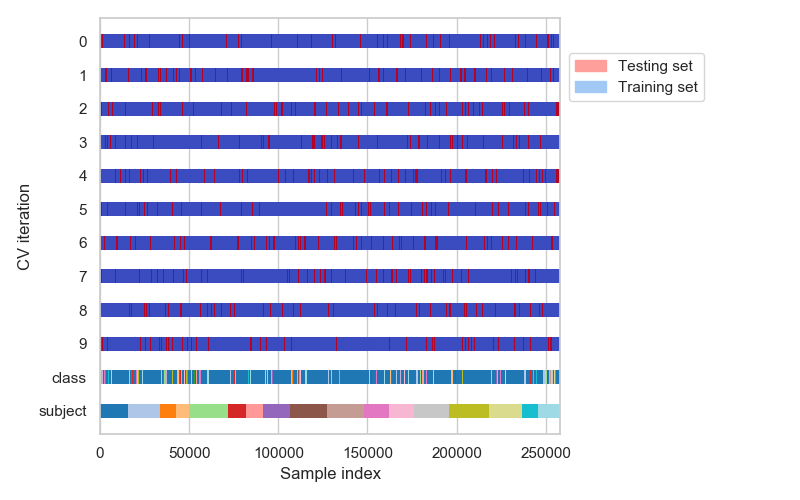
\includegraphics[width=.5\textwidth]{Figures/ShuffleSplit.png}
    \caption{10-CV process in overlapping windowed dataset by window size=.5 s }
    \label{fig:Shuffle-cv}
\end{figure}

\end{itemize}

We reproduce their work with the same dataset and improve it by applying overlapping sliding window approach instead of non-overlapping in segmentation stage and subject CV as an alternative for classic k-fold CV. In the next section, the dataset and methodology are explained precisely.

\section{Experiment setting}

\subsection{Dataset} \label{sec:dataset}
It is very important to use an adequate representative dataset to evaluate the impact of window size on the performance of the classifier in the recognition process. In this paper, one of the most complete human activity recognition dataset \cite{banos2012benchmark} in terms of the number of considered activities and subjects is used. This dataset is composed of data collected from 17 subjects of diverse profiles while wearing 9 Xsens inertial measurement units on different parts of their body and perform 33 fitness activities [Table \ref{tab:Activites}] ranging from Warm up to fitness exercises in an out-of-lab environment. Each sensor node provides tri-directional acceleration, gyroscope, and magnetic field
measurements as well as orientation estimates in quaternion format (4D). Although using several sensors help to capture the body dynamics, here only the acceleration data is used to study. This dataset provides data for three sensor displacement scenarios to compare the sensor anomalies(out of the scope of this work); thus, only the data from default scenario is used.

%  start of Table1
\begin{table}[h!]
\tiny  
  \centering
\begin{tabular}{|c|c|}
\hline 
\multicolumn{2}{|c|}{Activities}\tabularnewline
\hline 
\hline 
Walking (1 min) & Upper trunk and lower body opposite twist (20x)\tabularnewline
\hline 
Jogging (1 min) & Arms lateral elevation (20x)\tabularnewline
\hline 
Running (1 min) & Arms frontal elevation (20x)\tabularnewline
\hline 
Jump up (20x) & Frontal hand claps (20x)\tabularnewline
\hline 
Jump front \& back (20x) & Arms frontal crossing (20x)\tabularnewline
\hline 
Jump sideways (20x) & Shoulders high amplitude rotation (20x)\tabularnewline
\hline 
Jump leg/arms open/closed (20x) & Shoulders low amplitude rotation (20x)\tabularnewline
\hline 
Jump rope (20x) & Arms inner rotation (20x)\tabularnewline
\hline 
Trunk twist (arms outstretched) (20x) & Knees (alternatively) to the breast (20x)\tabularnewline
\hline 
Trunk twist (elbows bended) (20x) & Heels (alternatively) to the backside (20x)\tabularnewline
\hline 
Waist bends forward (20x) & Knees bending (crouching) (20x)\tabularnewline
\hline 
Waist rotation (20x) & Knees (alternatively) bend forward (20x)\tabularnewline
\hline 
Waist bends (reach foot with opposite hand) (20x) & Rotation on the knees (20x)\tabularnewline
\hline 
Reach heels backwards (20x) & Rowing (1 min)\tabularnewline
\hline 
Lateral bend (10x to the left + 10x to the right) & Elliptic bike (1 min)\tabularnewline
\hline 
Lateral bend arm up (10x to the left + 10x to the right) & Cycling (1 min)\tabularnewline
\hline 
Repetitive forward stretching (20x) & \tabularnewline
\hline 
\end{tabular}

      % Title of the table
        \caption{Activity set }
        \label{tab:Activites}

\end{table} 

%  end of Table1

\subsection{Study setup}
In this section the setting of our work for ARP which was explained before in Section \ref{subsec:ARP} is clarified. Like \cite{banos2014window} in this work no preprocessing is applied to the dataset. As for segmentation stage, the overlapping sliding window technique sliding at 200 ms for diverse window sizes ranging from .25 s to 7 s is used (i.e., each 5s window shares 4.8s of data with the previous window). Regarding the feature extraction step, the same feature sets as \cite{banos2014window} are considered. Finally, for the classification part, several powerful and common machine learning models are selected for discrimination of activities: Decision Tree (DT),k-nearest neighbors(KNN, K=3), Naive Bayes (NB), Nearest centroid classifier (NCC), Random forest(RF)and Logistic regression classifier(LR).We used these classifiers as implemented in scikit-learn 0.20 \cite{pedregosa2011scikit}.\newline

Here, in order to evaluate the model performance under different window sizes, we use a subject CV process (see Section \ref{sub:subjective CV} for explanation).

As can be seen in Figure \ref{fig:class}, the dataset is extremely imbalance meaning that there are more data-points for some classes(activities)in the dataset. Under such circumstances, the F1-score which conveys the balance between the precision and the recall is an appropriate metric for evaluating the performance of the models. It reaches its best value at 1 (perfect precision and recall) and worst at 0.

% figure 2
\begin{figure}[h]
    \centering
    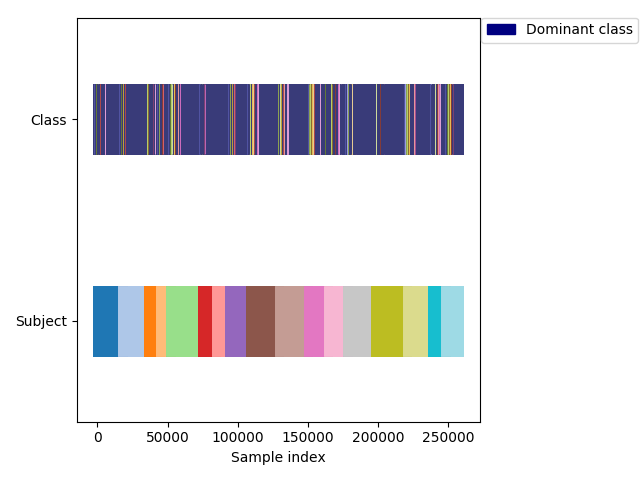
\includegraphics[width=.4\textwidth]{Figures/Class_subject.png}
    \caption{Example of distribution of activities and subjects in overlapping windowed dataset with window size=.5 s.The class 0 which means doing nothing accounts for more than 72 percent of the classes.Each color represents different activities and subjects in "Class" and "Subjects" respectively.}
    \label{fig:class}
\end{figure}

\subsection{Subject cross-validation process} \label{sub:subjective CV}
As mentioned before in section \ref{sec:dataset}, the used dataset in this study comprises the observations of 17 subjects with diverse profiles; consequently, such dataset is likely to be dependent on individual subjects. Under such circumstances, a safe approach to know the performance of the model is training on a particular set of subjects data and validate on the unseen ones in order to know how the trained model generalizes well on different groups. Although this method might be time-consuming (especially when the number of subjects is high), it is a very encouraging way to evaluate the domain-specific datasets. As can be seen in Figure \ref{fig:Subjective-cv}, in each fold the model trained on all groups except one which is used for testing.

% figure 4
\begin{figure}[h]
    \centering
    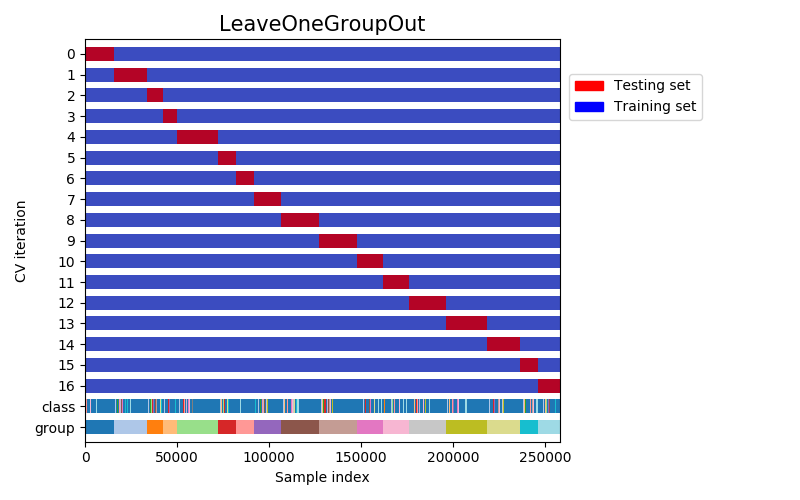
\includegraphics[width=.5\textwidth]{Figures/LeaveOneGroupOut.png}
    \caption{17-SCV process in overlapping windowed dataset by window size=.5 s- here there are 17 subjects in the dataset,consequently 17 folds  }
    \label{fig:Subjective-cv}
\end{figure}


\section{Results}

In this section, the performance of models for diverse window sizes is examined.Figure \ref{fig:NO-iid-results}, \ref{fig:O-iid-results}, \ref{fig:NO-subjective-results} and \ref{fig:O-subjective-results} indicate the impact of different window size on the recognition performance (F1-score) of several classifiers for the combination of two sliding window techniques (non-overlapping and overlapping) and two cross-validation processes (subject and i.i.d).At the first glance, it can be seen that the performance of the models improves as the feature set becomes richer, particularly FS2 which notably empowers the classifiers such as NC and NB in comparison with FS1. The differences among the results for FS1,FS2, and FS3 may show that having more features may lead to better performances. Overall, window size= 1 s was a "cut-off" for all scenarios and from this values on, no significant benefit was obtained.\newline

In the Non-overlapping windowing of i.i.d CV (Figure \ref{fig:NO-iid-results} ), in general, the performance of KNN, DT and RF models showed a downward trend as the size of window rose. The optimal window size for DT and RF models was the same in FS1 and FS2 at .25 s and 1.25 s respectively, but it was different in FS3. As for KNN, it ranked first among all models for all feature sets with the F1-score above 0.96 for FS1 and FS2 and almost 0.96 for FS3. This classifier allows us to maximally decline the window size. While the size of window grew, there was a slight fluctuation in the performance of RF. It peaked at window size 1.5 s for FS1 and 1.25 s for FS2 and FS3.In general, the performance of NB and NC models , except for FS3-NC, went up as the size of window increased. In particular, enlarging the window size by 1 s was resulted in rising up to 50\% and 30\% for NC and NB models respectively.
 \newline
By contrast, as Figure \ref{fig:O-iid-results} represents, while the size of window climbed, the performance of KNN, DT, LR and RF rose in general. Although the correlation between optimal window size for DT and RF was the same as before (equal for FS1 and FS2 and varying for FS3), here it enlarged tremendously and overall, they needed the largest window size among all models for all feature sets. However, this change was gradual for LR model. KNN like before stood out among all model for all feature sets, but it no longer was the best in terms of optimal window size.NB and NC showed a similar trend to non-overlapping and they reached to the best F1-score between 1 s and 2 s and generally needed shortest window size for that.\newline

In the subject CV (Figure \ref{fig:NO-subjective-results}), KNN, LR, RF and DT models showed a similar trend and surprisingly, their classification performance dropped substantially and never reached the F1-score above 90 \%. However, for NB and NC the performance remained unchanged. Here, broadly as the window size increased, the F1-score of KNN, LR, RF, and DT fell slowly and went up for NB and NC.KNN model in terms of performance and shorter window size placed the first among all models.LR and RF at most needed 1 s window size to hit their peaks.



\begin{figure*}[htp]
  \centering
  \subfigure[FS1]{
\label{fig:NO-FS1-iid}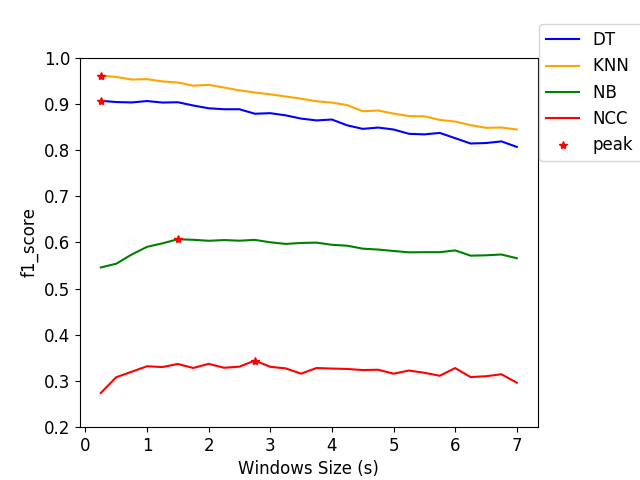
\includegraphics[scale=0.355]{Figures/FS1-iid-splitting-non-overlapping.png}}\quad
  \subfigure[FS2]{\label{fig:NO-FS2-iid}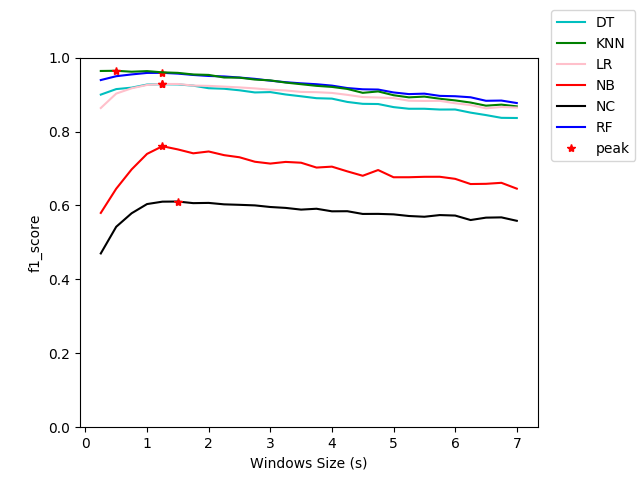
\includegraphics[scale=0.355]{Figures/FS2-iid-splitting-non-overlapping.png}}
  \subfigure[FS3]{\label{fig:NO-FS3-iid}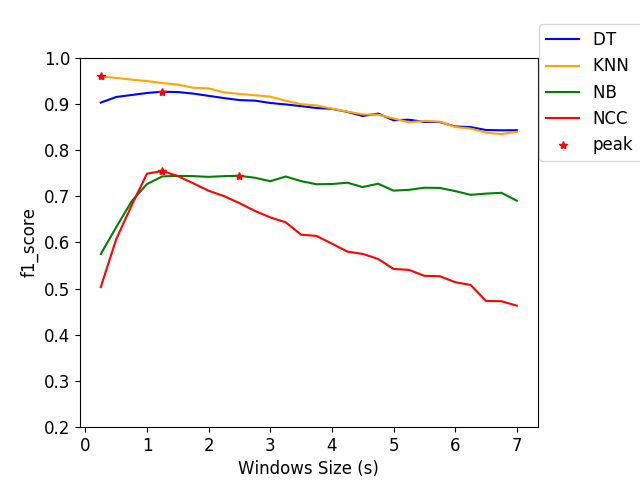
\includegraphics[scale=0.355]{Figures/FS3-iid-splitting-non-overlapping.png}}
   
   \caption{Non-overlapping windowing-i.i.d CV}
   \label{fig:NO-iid-results}
\end{figure*}

\begin{figure*}[htp]
  \centering
  \subfigure[FS1]{
\label{fig:O-FS1-iid}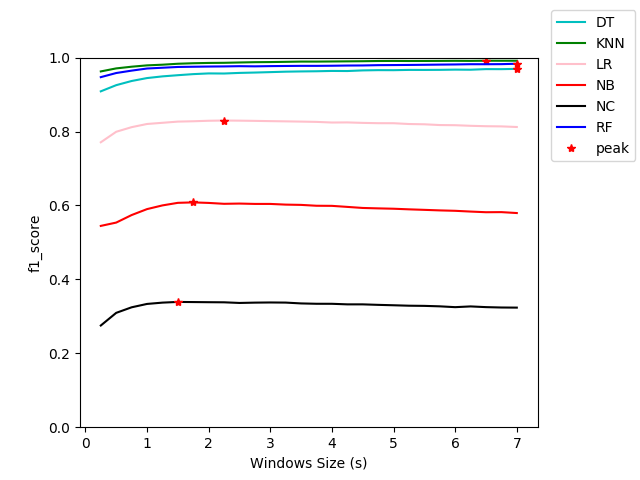
\includegraphics[scale=0.355]{Figures/FS1-iid-splitting-overlapping.png}}\quad
  \subfigure[FS2]{\label{fig:O-FS2-iid}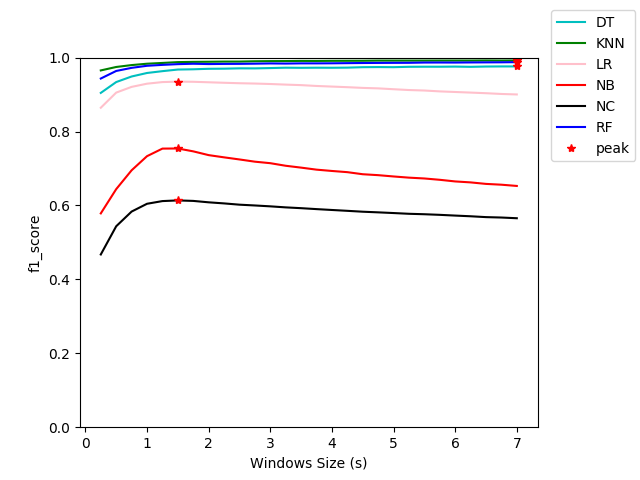
\includegraphics[scale=0.355]{Figures/FS2-iid-splitting-overlapping.png}}
  \subfigure[FS3]{\label{fig:O-FS3-iid}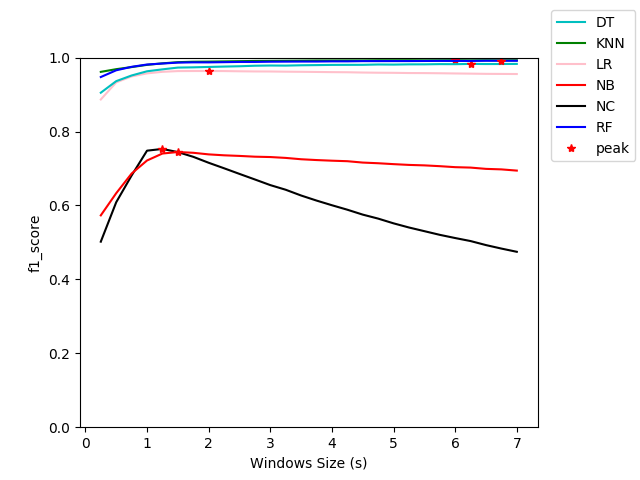
\includegraphics[scale=0.355]{Figures/FS3-iid-splitting-overlapping.png}}
   
   \caption{Overlapping windowing-i.i.d CV}
    \label{fig:O-iid-results}

\end{figure*}

\begin{figure*}[htp]
  \centering
  \subfigure[FS1]{
\label{fig:NO-FS1-sbj}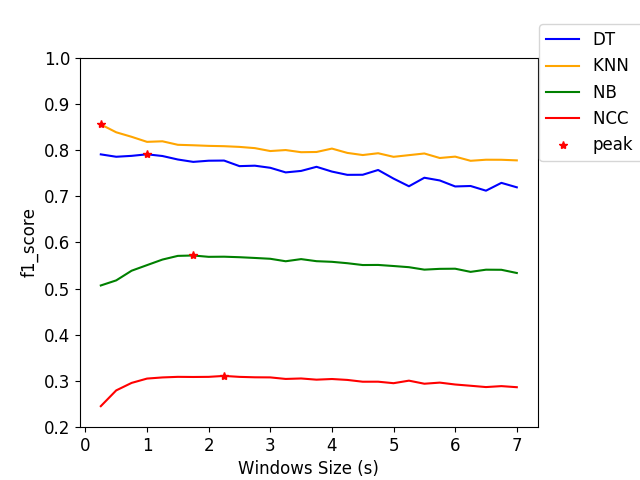
\includegraphics[scale=0.355]{Figures/FS1-subjective-splitting-non-overlapping.png}}\quad
  \subfigure[FS2]{\label{fig:NO-FS2-sbj}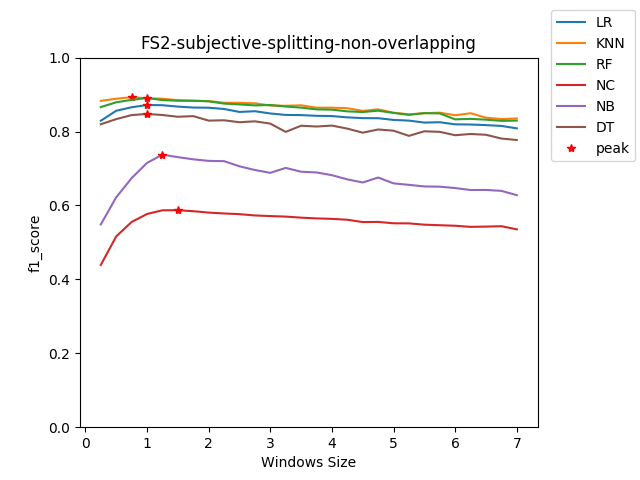
\includegraphics[scale=0.355]{Figures/FS2-subjective-splitting-non-overlapping.png}}
  \subfigure[FS3]{\label{fig:NO-FS3-sbj}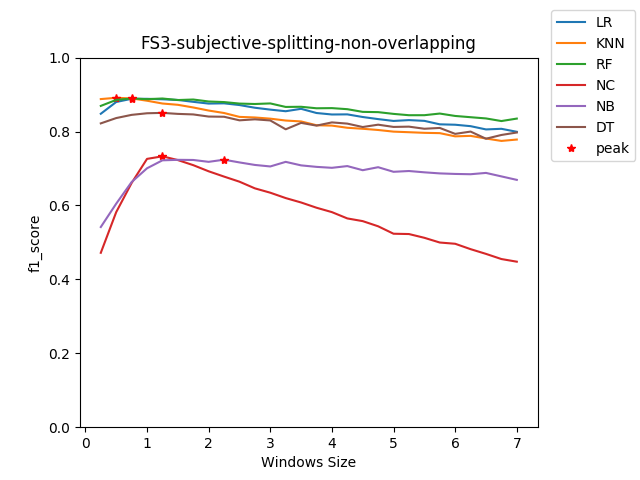
\includegraphics[scale=0.355]{Figures/FS3-subjective-splitting-non-overlapping.png}}
   
   \caption{Non-overlapping windowing-subject CV}
    \label{fig:NO-subjective-results}

\end{figure*}


\begin{figure*}[htp]
  \centering
  \subfigure[FS1]{
\label{fig:O-FS1-sbj}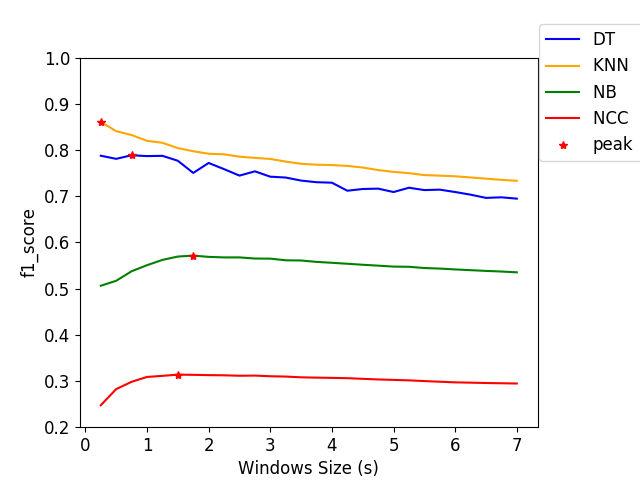
\includegraphics[scale=0.355]{Figures/FS1-subjective-splitting-overlapping.png}}\quad
  \subfigure[FS2]{\label{fig:O-FS2-sbj}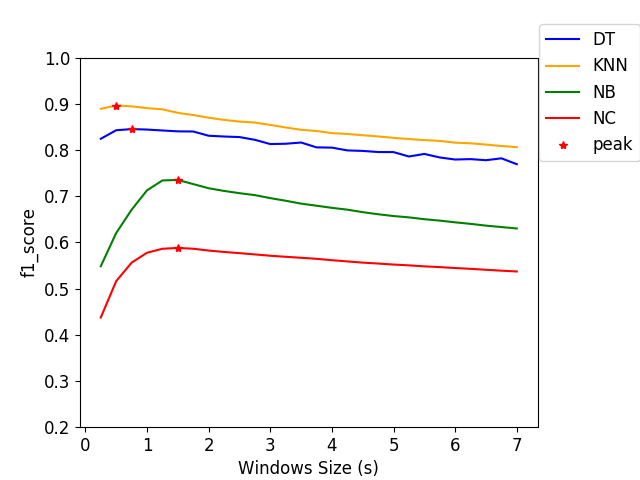
\includegraphics[scale=0.355]{Figures/FS2-subjective-splitting-overlapping.png}}
  %\subfigure[FS3]{\label{fig:O-FS3-sbj}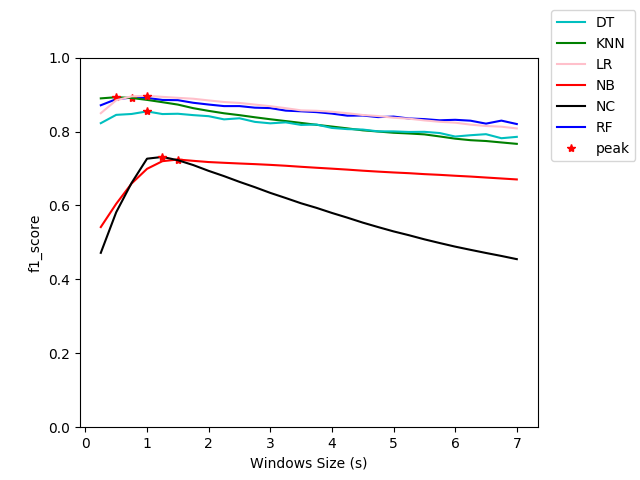
\includegraphics[scale=0.355]{Figures/FS3-subjective-splitting-overlapping.png}}
   
   \caption{Overlapping windowing-subject CV}
    \label{fig:O-subjective-results}

\end{figure*}












\section{Discussion}



\section{Conclusions}
--------------------------
%\end{document}  % This is where a 'short' article might terminate




\begin{acks}

-----------
\end{acks}
